\begin{exercise}
		Να εφαρμοστεί ο αλγόριθμος Bresenham για τις ευθείες :
	\begin{enumerate}
		\item[$\mathrm{i)}$] $P_1(1, 1) \to P_2(3, 2)$
		\item[$\mathrm{ii)}$] $P_1(1, 1) \to P_2(4, 13)$
		\item[$\mathrm{iii)}$] $P_1(0, 0) \to P_2(0, 10)$	
	\end{enumerate}
	
	Να συγκριθούν οι πολυπλοκότητες σε σχέση με τον αλγόριθμο Plotline.	
\end{exercise}

\begin{solution}
	
\textcolor{red}{Θέλει ΔΙΟΡΘΩΣΗ}


\begin{enumerate}
    \item[$\mathrm{i)}$] $P_1(1, 1) \to P_2(3, 2)$
    
    \begin{itemize}
        \item $Dx = x_2 - x_1 = 3 - 1 = 2$
        \item $Dy = y_2 - y_1 = 2 - 1 = 1$
        \item $x = x_1  = 1$, $y = y_1 = 1$
        \item $c_1 = 2 \cdot Dx = 2 \cdot 2 = 4$
        \item $error = c_1 - Dy = 4 - 1 = 3$
        \item $c_2 = error - Dy = 3 - 1 = 2$
     \end{itemize}

Εφόσον $y_2 = 2$, από την επανάληψη θα έχουμε:
        
        \begin{itemize}
            \item \underline{$y = 1 \leq 2$} \newline 
            Τότε $error = 3 \geq 0$. Άρα: \newline 
            $x= x+1 = 2$ και $error = error + c_2 = 3 + 2 = 5$
            Φωτίζεται το pixel $(2,2)$ και $y = y+1 = 2$.
            \item \underline{$y = 2 \leq 2$} \newline 
             Τότε $error = 5 \geq 0$. Άρα  \newline 
            $x= x+1 = 3$ και $error = error + c_2 = 5 + 2 = 7$
            Φωτίζεται το pixel $(3,2)$ και $y = y+1 = 3$.
            \item \underline{$y = 3 > 2$} άρα ο αλγόριθμος σταματάει.
        \end{itemize}
Συνολικά θα φωτιστούν τα σημεία : $(1, 1), (2, 2), (3, 2)$.

\begin{figure}[hbt]
	\begin{center}
	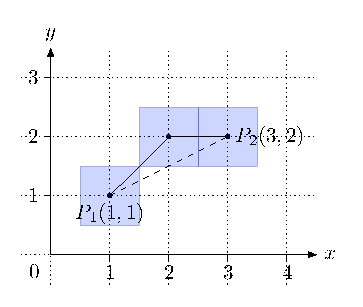
\includegraphics[scale=0.8]{Chapter1/Exercises/ex4/graph1.pdf}
	\end{center}
\caption{Γραφική λύση ευθείας Bresenham: $P_1(1, 1) \to P_2(3, 2)$}
\end{figure}
    
\item[$\mathrm{ii)}$] $P_1(1, 1) \to P_2(4, 13)$
    

    \begin{itemize}
        \item $Dx = x_2 - x_1 = 4 - 1 = 3$
        \item $Dy = y_2 - y_1 = 13 - 1 = 12$
        \item $x = 1$, $y = 1$
        \item $c_1 = 2 \cdot Dx = 2 \cdot 3 = 6$
        \item $error = c_1 - Dy = 6 - 12 = -6$
        \item $c_2 = error - Dy = -6 - 12 = -18$
	\end{itemize}   
        
         
Εφόσον $y_2 = 13$, από την επανάληψη θα έχουμε:     
       
        \begin{itemize}
            \item \underline{$y = 1 \leq 13$} \newline 
            Τότε $error = -6 < 0$. Άρα: \newline 
			$error = error + c_1 = - 6 + 6 =0 $
            Φωτίζεται το pixel $(1,1)$ και $y = y+1 = 2$.
            
            \item \underline{$y = 2 \leq 13$} \newline 
            Τότε $error = 0 \geq 0$. Άρα: \newline 
            $x= x+1 = 2$ και $error = error + c_2 = 0 - 18$.
            Φωτίζεται το pixel $(2,2)$ και $y = y+1 = 3$.
            
            \item \underline{$y = 3 \leq 13$} \newline 
				 Tότε:  
            $error = -18 < 0$. Άρα: \newline  
            $error = -18 + 6 = -12$. 
            Φωτίζεται το pixel $(2,3)$ και $y = y+1 = 4$.
            \item Κ.ο.κ. έως ότου: $y = 13$.
        \end{itemize}
Συνολικά θα φωτιστούν τα σημεία: \newline  $(1, 1), (1, 2), (1, 3), (1, 4), (2, 5), (2, 6), (2, 7), (3, 8), (3, 9), (3, 10), (3, 11), (4, 12), (4, 13)$.
    
\item[$\mathrm{iii)}$] $P_1(0, 0) \to P_2(0, 10)$
    
    \begin{itemize}
        \item  $Dx = x_2 - x_1 = 0 - 0 = 0$
        \item  $Dy = y_2 - y_1 = 10 - 0 = 10$
        \item  $x = 0$, $y = 0$
        \item  $c_1 = 2 \cdot Dx = 2 \cdot 0 = 0$
        \item  $error = c_1 - Dy = 0 - 10 = -10$
        \item  $c_2 = error - Dy = -10 - 10 = -20$
	\end{itemize}   
	
Εφόσον $y_2 = 10$, από την επανάληψη θα έχουμε:    

        \begin{itemize}
            \item \underline{$y = 0 \leq 10$}  \newline 
            Τότε $error = -10 < 0$. Άρα: \newline 
			$error = error + c_1 = -10 + 0 = -10$           
			Φωτίζεται το pixel $(0,0)$ και $y = y+1 = 1$.

            \item \underline{$y = 1 \leq 10$}  \newline 
            Τότε $error = -10 < 0$. Άρα: \newline
            $error = -10 + 0 = -10$. Φωτίζεται το pixel $(0,1)$ και $y = y+1 = 2$.
            \item  Κ.ο.κ. έως ότου: $y = 10$.
        \end{itemize}
Συνολικά θα φωτιστούν τα σημεία: \newline $(0, 0), (0, 1), (0, 2), (0, 3), (0, 4), (0, 5), (0, 6), (0, 7), (0,8), (0,9), (0, 10)$.


\begin{figure}[h!]
	\begin{minipage}[b]{0.48\textwidth} % Top-left image	
		\begin{center}
		   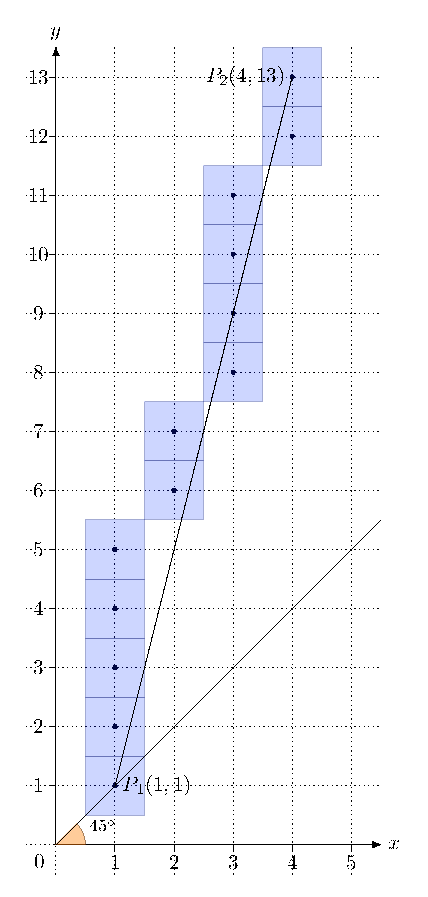
\includegraphics[scale=0.8]{Chapter1/Exercises/ex4/graph2.pdf}
		\end{center}    
		\captionof{figure}{Γραφική λύση ευθείας Bresenham: $P_1(1, 1) \to P_2(4, 13)$}
	\end{minipage}%
	\hfill
	\begin{minipage}[b]{0.48\textwidth} % Top-right image
	    \begin{center}
		    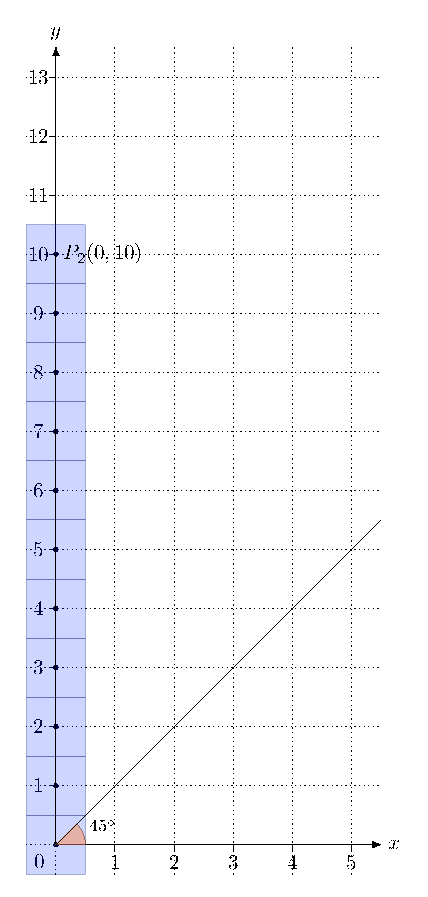
\includegraphics[scale=0.8]{Chapter1/Exercises/ex4/graph3.pdf}
		\captionof{figure}{Γραφική λύση ευθείας Bresenham: $P_1(0, 0) \to P_2(0, 10)$}
		\end{center}    
	\end{minipage}

\end{figure}
		

Η πολυπλοκότητα του αλγορίθμου του Bresenham είναι σαφώς χαμηλή, σε σχέση με τον αλγόριθμο Plotline. Η εισαγωγή της επιπλέον μεταβλητής \texttt{error} απαλλάσσει τον αλγόριθμο από πολλαπλασιασμούς, ενώ επιπλέον δεν απαιτείται στρογγύλευση.

\end{enumerate}



\end{solution}
